\providecommand{\main}{..} 
\documentclass[\main/boa.tex]{subfiles}

\begin{document}

\section{Text mining w R}
\begin{minipage}[t]{0.915\textwidth}
	\center     
    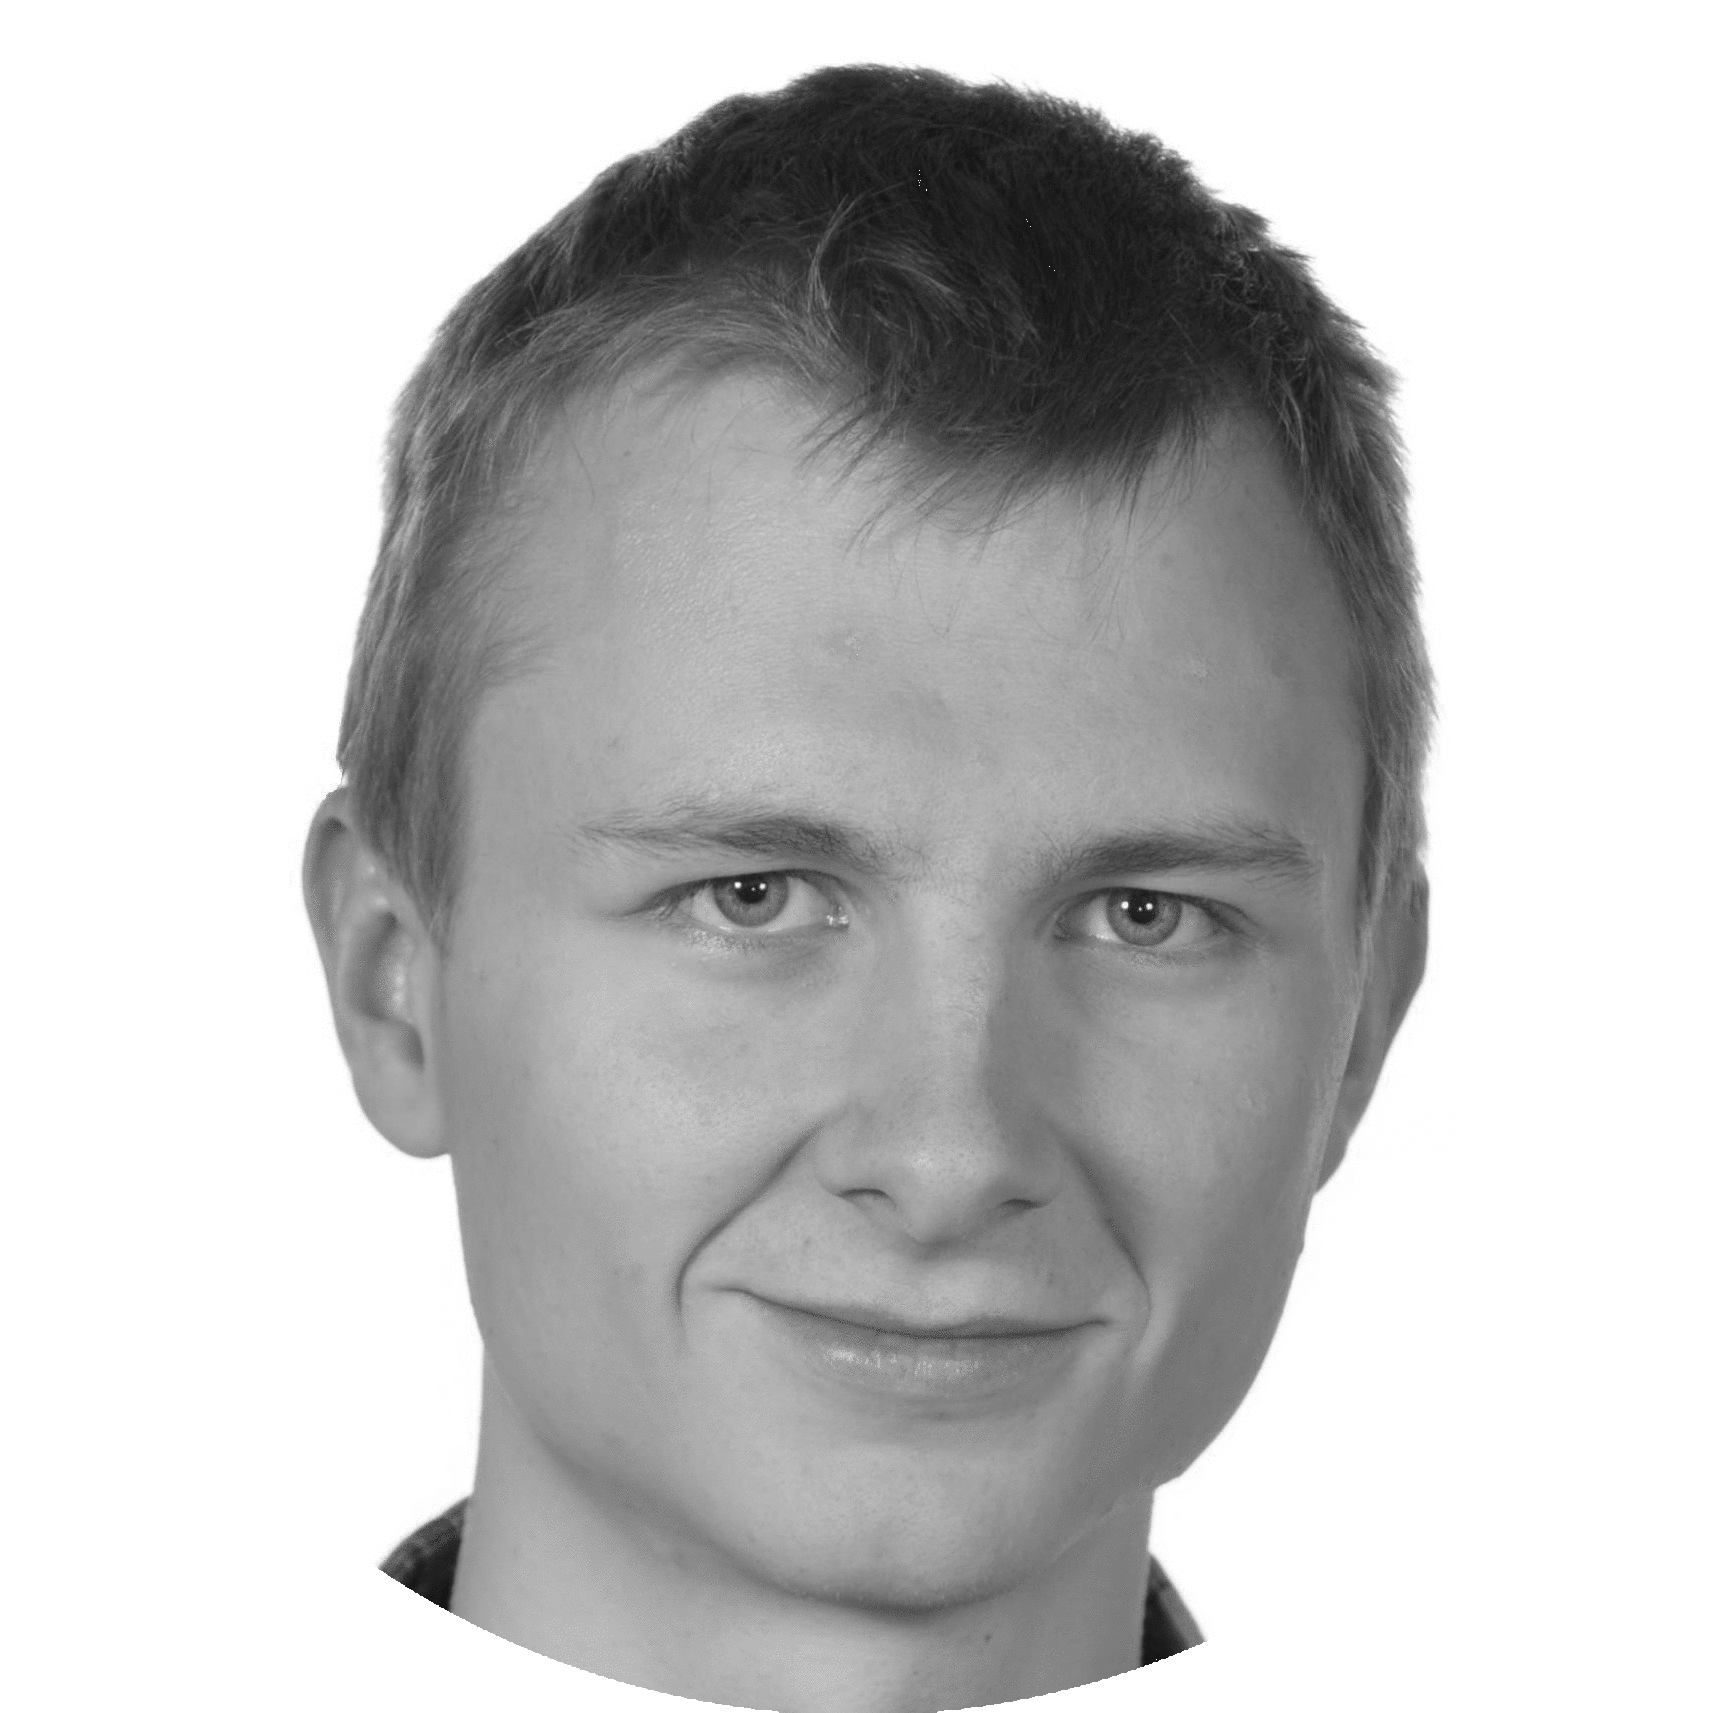
\includegraphics[width=60px]{img/workshops/czarno_biale/ryciak-crop.png} 
\end{minipage}

\begin{minipage}{0.915\textwidth}
\centering
{\bf \index[a]{Ryciak Norbert} Norbert Ryciak}
\end{minipage}

\vskip 0.3cm

\begin{affiliations}
\begin{minipage}{0.915\textwidth}
\centering
\large Politechnika Warszawska, Wydział MiNI  \\[2pt]
\end{minipage}
\end{affiliations}

\vskip 0.8cm

\opiswarsztatu Celem warsztatu jest zapoznanie uczestników z podstawowymi technikami stosowanymi podczas analizy tekstu. Omówione zostanie m. in. zagadnienie modelowania tematycznego przy użyciu modelu LDA. Duży nacisk będzie położony na poznanie specyfiki pracy z danymi tekstowymi i zrozumienie motywacji prowadzących do określonych metod analizy. Wybrane zagadnienia zostaną zaprezentowane w zastosowaniu do grupowania lub klasyfikacji tekstów.

\planwarsztatu
\begin{enumerate}
\item Wstępne przetwarzanie i redukcja wymiaru danych
\item Podstawowe metody reprezentacji zbioru danych tekstowych
\item Modelowanie tematyczne - model LDA (Latent Dirichlet Allocation)
\end{enumerate}	 

\end{document}